\documentclass{beamer}
 
\usepackage{beamerthemesplit}
\usepackage[utf8]{inputenc} 
\usepackage[russian]{babel}
\usepackage{amsmath,amssymb}
\usepackage{graphicx}
\usepackage{subfigure}
\usepackage{amsthm}
 
 
\newtheorem{thm}{Теорема}
\newtheorem{lem}[thm]{Лемма}
\newtheorem{defn}{Определение}
\newtheorem{exmpr}{Использование в R}
\newtheorem{exmp}{Пример}

\date{\today}
 
\begin{document}
\title[\hspace{15em}\insertframenumber/\inserttotalframenumber]{Лекция 1. Основы математической статистики.}
\begin{frame}
  \titlepage
\end{frame}
 
 
\begin{frame}
\frametitle{Случайные выборки}
\begin{defn}Случайная выборка размера $n$, отвечающая случайной величине X с функцией распределения $F(x)$ - набор $n$ независимых случайных величин $X_1,\ldots,X_n$, имеющих функцию распределения $F(x)$.
\end{defn}
\begin{defn}
Статистика - функция случайной выборки.
\end{defn}
\end{frame}
 
\begin{frame}[containsverbatim]
\frametitle{Эмпирическая функция распределения}
%\begin{center}
%\includegraphics[width=0.8\textwidth,height=0.8\textheight]{EMC_HK187720907.jpg}
%\end{center}
\begin{defn}
Эмпирическая функция распределения:
$$F_n(x)=\frac{1}{n}\sum_{l=1}^n{\mathbf{1}_{(-\infty,x)}(X_l)}$$
\end{defn}
\begin{thm}[Гливенко]
$\sup_{x\in \mathbb{R}}{|F_n(x)-F(x)|}\xrightarrow[n\rightarrow\infty]{}0$ с вероятностью 1
\end{thm}
\begin{exmpr}
\begin{verbatim}
> set.seed(1);x <- rnorm(1000)
> ecdfx <- ecdf(x)
> plot(ecdfx)
\end{verbatim}
\end{exmpr}
\end{frame}

\begin{frame}[containsverbatim]
\frametitle{Гистограмма}
\begin{defn}
Эмпирическая плотность распределения(гистограмма):
$$f_{n,h}(x)=\frac{1}{nh}\sum_{l=1}^n{\mathbf{1}_{(x_h,x_h+h)}(X_l)}$$
где $x_h=[x/h]h$
\end{defn}
\begin{thm}
Если $n\rightarrow \infty$, $h\rightarrow 0$, $nh\rightarrow\infty$, то $\forall x$, таких, что $f(x)$ - непрерывна, $f_{n,h}(x)\rightarrow f(x)$ по вероятности.
\end{thm}
\begin{exmpr}
\begin{verbatim}
> h <- hist(x)
\end{verbatim}
\end{exmpr}

\end{frame}


\begin{frame}[containsverbatim]
\frametitle{Оценки параметров распределения}
\begin{defn}[Выборочное среднее]
$$\overline{X}_n=\frac{1}{n}\sum_{l=1}^n{X_l}$$
\end{defn}
\begin{defn}[Выборочная дисперсия]
$$S_n^2=\frac{1}{n-1}\sum_{l=1}^n{(X_l-\overline{X}_n)^2}$$
\end{defn}
\begin{exmpr}
\begin{verbatim}
> m <- mean(x)
> v <- var(x)
\end{verbatim}
\end{exmpr}
\end{frame}

\begin{frame}[containsverbatim]
\frametitle{Коэффициент корреляции}
\begin{defn}[Выборочный коэффициент корреляции]
$$R_n=\frac{\sum_{l=1}^n{(X_l-\overline{X})(Y_l-\overline{Y})}}{\sqrt{S_n^2(X)S_n^2(Y)}}$$
\end{defn}
\begin{columns}
\column{0.5\textwidth}
\begin{exmpr}
\begin{verbatim}
> corx <- cor(x)
\end{verbatim}
\end{exmpr}
\column{0.5\textwidth}
\begin{center}
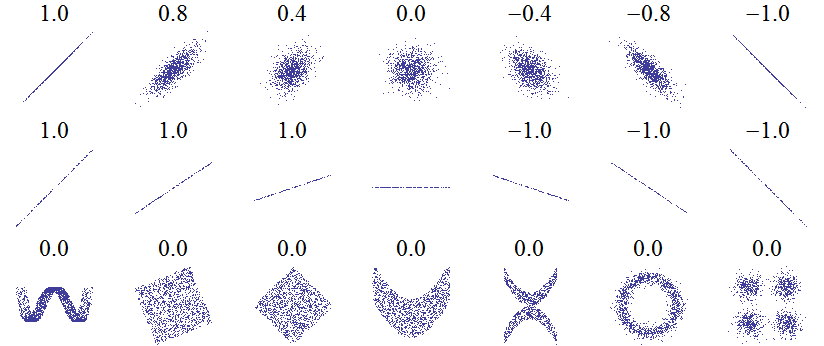
\includegraphics[width=1\textwidth,height=0.35\textheight]{correlation_examples.png}
\end{center}
\end{columns}

\end{frame}

\begin{frame}
\frametitle{Доверительные интервалы}
\begin{defn}[Доверительный интервал]
Интервал $(\underline{\theta}(X_1,\ldots,X_n),\overline{\theta}(X_1,\ldots,X_n))$ называется доверительным для параметра $\theta$ с уровнем значимости $\alpha$, если
$$P(\underline{\theta}(X_1,\ldots,X_n)<\theta<\overline{\theta}(X_1,\ldots,X_n))\geq 1-\alpha$$
\end{defn}
\end{frame}

\begin{frame}
\frametitle{Доверительные интервалы}
\begin{exmp}
Легко показать, что для выборки из нормального распределения $\mathrm{N}(\theta,\sigma^2)$
$$\sqrt{n} \cdot \frac{\overline{X}_n - \theta}{\sigma} \sim \mathrm{N}(0,1)$$
Таким образом, доверительный интервал для параметра $\theta$ будет
$$(\overline{X}_n-\frac{z_{1-\frac{\alpha}{2}}\sigma}{\sqrt{n}},\overline{X}_n+\frac{z_{1-\frac{\alpha}{2}}\sigma}{\sqrt{n}})$$
\end{exmp}
\end{frame}

\begin{frame}
\frametitle{Проверка статистических гипотез}
\begin{defn}
$X_1,\ldots,X_n\sim F(x,\theta)$, $\theta \in \Theta=\Theta_0\cup\Theta_1$, $\Theta_0\cap\Theta_1=\emptyset$\\
Нулевая гипотеза $H_0$: $\theta \in \Theta_0$\\
Альтернативная гипотеза $H_1$: $\theta \in \Theta_1$\\
Статистический критерий - правило, позволяющее отвергнуть или принять нулевую гипотезу.
\end{defn}
\begin{defn}
Вероятность ошибки первого рода $\alpha$ - вероятность отвергнуть гипотезу $H_0$ при условии, что она верна.
\end{defn}
\begin{defn}
Вероятность ошибки второго рода - вероятность принять гипотезу $H_0$ при условии, что верна гипотеза $H_1$.
\end{defn}

\end{frame}

\begin{frame}
\frametitle{Проверка статистических гипотез}
\begin{exmp}
Есть выборка $X_1,\ldots,X_n\sim\mathrm{N}(\theta,\sigma^2)$, где $\sigma^2$ - известный параметр, а $\theta$ - неизвестный. \\Хотим проверить гипотезу $\theta=\theta_0$.\\
Посчитаем следующую статистику:
$$\sqrt{n} \cdot \frac{\overline{X}_n - \theta_0}{\sigma}$$
Если $\theta=\theta_0$, то эта статистика имеет распределение $\mathrm{N}(0,1)$.
Таким образом, если в качестве статистического критерия рассмотреть попадание в доверительный интервал $$(\overline{X}_n-\frac{z_{1-\frac{\alpha}{2}}\sigma}{\sqrt{n}},\overline{X}_n+\frac{z_{1-\frac{\alpha}{2}}\sigma}{\sqrt{n}}),$$
то вероятность ошибки первого рода будет $\alpha$.
\end{exmp}

\end{frame}

\begin{frame}
\frametitle{Проверка статистических гипотез}
\begin{exmp}
Машина должна заполнять упаковку веществом на 250 грамм. Задача: имея выборку из 25 упаковок, проверить  с уровнем значимости 0.05, правильно ли откалибрована машина. Ранее было оценено, что распределение заполнения вещества нормально со средним отклонением 2.5 грамма.
\begin{center}
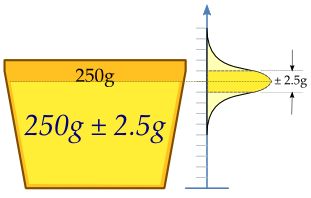
\includegraphics[width=0.5\textwidth,height=0.35\textheight]{margarinefilling.png}
\end{center}  
Правильно ли откалибрована машина, если среднее значение выборки 251 грамм?
\end{exmp}

\end{frame}


\begin{frame}
\frametitle{Проверка статистических гипотез}
\begin{defn}[P-значение]
Пусть есть случайная выборка и некоторая статистика с известным распределением.\\
Обычно (!), P-значение - это вероятность того, что случайная величина, имеющая то же распределение, что и статистика, примет значение, большее(в случае двустороннего распределения, возможно, и меньшее) фактического значения статистики на данной выборке.\\
P-значение следует сравнивать с каким-нибудь заранее выбранным порогом, например 0.05. Если оно меньше, то нулевая гипотеза отвергается.
\end{defn}

\end{frame}

\begin{frame}[containsverbatim]
\frametitle{Проверка гипотезы нормальности}
\begin{defn}[Статистика Шапиро-Уилка]
$$W=\frac{1}{s^2}\left[\sum_{i=1}^n a_{n-i+1} (x_{n-i+1} -x_i)\right]^2$$
\end{defn}
\begin{exmpr}
\begin{verbatim}
> shapiro.test(x)
	
    Shapiro-Wilk normality test
data:  x 
W = 0.9988, p-value = 0.7258
\end{verbatim}
\end{exmpr}
\end{frame}

\begin{frame}[containsverbatim]
\frametitle{Проверка гипотезы нормальности}
\begin{exmpr}[График квантиль-квантиль]
\begin{verbatim}
> qqnorm(x)
> qqline(x)
\end{verbatim}
\begin{center}
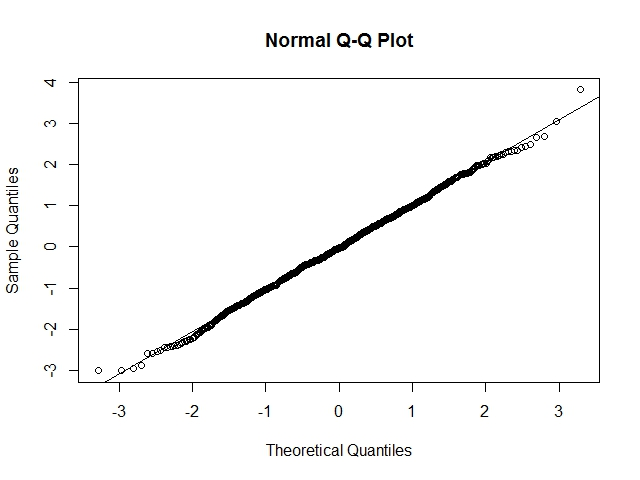
\includegraphics[width=0.8\textwidth,height=0.6\textheight]{qqnorm.jpeg}
\end{center}
\end{exmpr}
\end{frame}

\begin{frame}[containsverbatim]
\frametitle{Метод максимального правдоподобия}
\begin{defn}
$X_1,\ldots,X_n$ - случайная выборка с плотностью распределения $f(x,\theta)$. Оценкой максимального правдоподобия для $\theta$ называется 
$$\theta_n=\underset{\theta}{argmax} (f(X_1,\theta)\cdot\ldots\cdot f(X_n,\theta))$$
\end{defn}
\begin{exmpr}
\begin{verbatim}
> library("MASS")
> f <- fitdistr(x,"normal")
      mean           sd     
  -0.01164814    1.03439825 
 ( 0.03271054) ( 0.02312985)
\end{verbatim}
\end{exmpr}
\end{frame}
 
\end{document}
